\documentclass{beamer}

\usepackage{amsmath, amssymb, amstext}
\usepackage{fancyhdr}
\usepackage{algorithm}
\usepackage{algpseudocode}
\usepackage{mathtools}
\usepackage{tikz}
\usetikzlibrary[topaths]

\DeclarePairedDelimiter{\ceil}{\lceil}{\rceil}
\DeclarePairedDelimiter\floor{\lfloor}{\rfloor}

%Macros
\newcommand{\A}{\mathbb{A}} \newcommand{\C}{\mathbb{C}}
\newcommand{\D}{\mathbb{D}} \newcommand{\F}{\mathbb{F}}
\newcommand{\N}{\mathbb{N}} \newcommand{\R}{\mathbb{R}}
\newcommand{\T}{\mathbb{T}} \newcommand{\Z}{\mathbb{Z}}
\newcommand{\Q}{\mathbb{Q}}
 
 
\newcommand{\cA}{\mathcal{A}} \newcommand{\cB}{\mathcal{B}}
\newcommand{\cC}{\mathcal{C}} \newcommand{\cD}{\mathcal{D}}
\newcommand{\cE}{\mathcal{E}} \newcommand{\cF}{\mathcal{F}}
\newcommand{\cG}{\mathcal{G}} \newcommand{\cH}{\mathcal{H}}
\newcommand{\cI}{\mathcal{I}} \newcommand{\cJ}{\mathcal{J}}
\newcommand{\cK}{\mathcal{K}} \newcommand{\cL}{\mathcal{L}}
\newcommand{\cM}{\mathcal{M}} \newcommand{\cN}{\mathcal{N}}
\newcommand{\cO}{\mathcal{O}} \newcommand{\cP}{\mathcal{P}}
\newcommand{\cQ}{\mathcal{Q}} \newcommand{\cR}{\mathcal{R}}
\newcommand{\cS}{\mathcal{S}} \newcommand{\cT}{\mathcal{T}}
\newcommand{\cU}{\mathcal{U}} \newcommand{\cV}{\mathcal{V}}
\newcommand{\cW}{\mathcal{W}} \newcommand{\cX}{\mathcal{X}}
\newcommand{\cY}{\mathcal{Y}} \newcommand{\cZ}{\mathcal{Z}}

\author{Justin Toth}
\institute{University of Waterloo}
\date{March 1st, 2016}
\title{Stable Matching Polytope\\ and Iterative Rounding}

\begin{document}
\begin{frame}
\titlepage
\end{frame}

\AtBeginSubsection[]
{
	\begin{frame}<beamer>
		\frametitle{Outline}
		\tableofcontents[currentsection, currentsubsection]
	\end{frame}
}
\section{Iterative Rounding}
\subsection{Bipartite Matching}

\begin{frame}
\frametitle{Weighted Bipartite Matching Problem}
Let $G=(V, E)$ be a bipartite graph with bipartition $V = V_0 \dot\cup V_1$. 
\begin{itemize}
\item For each $e \in E$, assign a cost $c_e$
\item $M \subseteq E$ is a matching if $\delta(v) \cap M \leq 1$ for all $v \in V$
\item $M(v)$ denotes the vertex $v$ is matched to under $M$
\item Problem: Find a matching $M$ maximizing $\sum_{e\in M} c_e$.
\end{itemize}
\begin{figure}
\centering
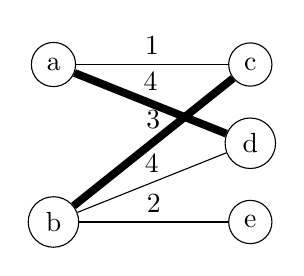
\begin{tikzpicture}
   \node[shape=circle,draw=black] (B) at (0,1) {b};
    \node[shape=circle,draw=black] (A) at (0,3) {a};
    \node[shape=circle,draw=black] (E) at (2.5,1) {e};
    \node[shape=circle,draw=black] (D) at (2.5,2) {d}; 
    \node[shape=circle,draw=black] (C) at (2.5,3) {c};

    \path[-] (A) edge node[above] {$1$} (C);
    \path [line width=1mm,-](A) edge node[above] {$4$} (D);
    \path [line width=1mm,-](B) edge node[above] {$3$} (C);
    \path [-](B) edge node[above] {$2$} (E);
    \path [-](B) edge node[above] {$4$} (D);

\end{tikzpicture}
\caption{A bipartite graph with edge weights. Optimal matching edges are thicker. $M(a) = d$}
\end{figure}
\end{frame}

\begin{frame}
\frametitle{Linear Programming Relaxation}
This problem can be formulated as a linear program, denoted $LP_M(G)$:
\begin{align*}
&\text{maximize} &\sum_{e \in E} c_e x_e \\
&\text{subject to} &x(\delta(v)) &\leq 1, &\forall v \in V\\
& &x_e &\geq 0, &\forall e \in E
\end{align*}
Where $x(\delta(v)) = \sum_{e \in \delta(v)} x_e$.
\end{frame}

\subsection{Integrality by Iterative Rounding}
\begin{frame}
\frametitle{Iterative Algorithm}
\begin{enumerate}
\item Input bipartite matching instance $G$
\item Set matching $M$ to $\emptyset$
\item While $E \neq \emptyset$
\begin{enumerate}
\item Find extreme point optimal solution $x$ to $LP_M(G)$.
\item For each $e=vw \in E$ such that $x_e = 1$ add $e$ to $M$ and remove vertices $v,w$ from $G$.
\item For each $e \in E$ such that $x_e = 0$ remove $e$ from $G$.
\end{enumerate}
\item Output $M$
\end{enumerate}
\end{frame}

\begin{frame}
\frametitle{Characterize Extreme Point Solution}
$\textbf{Rank Lemma:}$ The maximal number of linearly independent tight constraints at an extreme point is equal to the dimension of the polytope.\\
\uncover<2->{$\implies$\\
Let $x$ be an extreme point of $LP_M(G)$ such that $0<x<1$. Then there exists a set $W \subseteq V$ such that:
\begin{enumerate}
\item $|W| = |E|$
\item $x(\delta(v)) = 1$ for all $v \in W$
\item $\{\chi(\delta(v)) : v \in W \}$ is linearly independent
\end{enumerate}
where $\chi(\delta(v))$ denotes the incidence vector of $\delta(v)$.}
\end{frame}

\begin{frame}
\frametitle{Correctness - Finding $0$ or $1$}
\begin{itemize}
\item<1-> Suppose for contradiction we have an extreme point solution $x$ such that $0 < x < 1$
\item<2-> Choose $W \subseteq V$ with $|W| = |E|$ corresponding to a set of tight linearly independent constraints.
\item<3-> Will show $|E| > |W|$ by a Token Argument to obtain contradiction.
\end{itemize}
\end{frame}

\begin{frame}
\frametitle{Correctness - Finding $0$ or $1$ Token Argument}
\begin{itemize}
\item Give each edge a token.
\item Redistribute tokens to tight constraints.
\item Show after redistribution that all constraints have token and some edge has leftover.
\end{itemize}
\uncover<2->{We will redistribute according to the following rule:\\
\begin{enumerate}
\item Each edge $vw$ gives $\frac{1}{2}$ token to $v$ if $v \in W$ and gives $\frac{1}{2}$ token to $w$ if $w \in W$. 
\end{enumerate}}
\end{frame}

\begin{frame}
\frametitle{Correctness - Finding $0$ or $1$ Counting Tokens}
\begin{itemize}
\item<1->Each edge gives away $\leq 1$ token.
\item<2-> For any $v \in W$, $x(\delta(v)) = 1$ and each $x_e < 1$ implies $d(v) \geq 2$.
\item<3-> Each tight constraint receives $\geq 2 \cdot \frac{1}{2} = 1$ tokens.
\end{itemize}
\end{frame}

\begin{frame}
\frametitle{Correctness - Finding $0$ or $1$ Token Leftover}
\begin{itemize}
\item<1-> Since $G$ is bipartite: $\sum_{v \in V_0} \chi(\delta(v)) = \sum_{v \in V_1} \chi(\delta(v))$.
\item<2-> So there exists $v \not\in W$ (otherwise constraints in $W$ are not linearly independent).
\item<3-> Any $e \in \delta(v)$ does not give away all its tokens.
\item<4-> So $|E| > |W|$, a contradiction.
\end{itemize}
\end{frame}

\begin{frame}
\frametitle{Correctness - Optimality}
Let $M$ be matching returned. Let $x$ be optimal extreme point solution to $LP_M(G)$. Show $c(M) \geq c^Tx$ by induction on number of iterations of algorithm.
\begin{itemize}
\item<1-> If algorithm fixes $x_{vw} = 1$ during iteration then residual problem is: find a matching $M'$ on $G'=G-v-w$. Algorithm returns $M' \cup \{vw\}$.
\item<2-> $x' = x$ restricted to edges of $G'$ is feasible for $LP_M(G')$.
\item<3-> So $c(M' \cup \{vw\}) = c(M') + c_{vw} \geq c(x') + c_{vw} = c(x)$,
\item<4-> The case for fixing $x_{vw} = 0$ is similar.
\end{itemize}
\end{frame}

\begin{frame}
\frametitle{What do we get from this?}
Correct algorithm implies integrality of polytope:
\begin{itemize}
\item  From Linear Programming theory:  for extreme point $x$, there is a cost vector $c$, $x$ is unique optimal solution.
\item If $x$ is fractional, and we ran the algorithm with cost $c$ we would obtain an integral solution, $x^{Int}$ of equivalent cost.
\item Since $x^{Int}$ is feasible and $x^{Int} \neq x$ this contradicts uniqueness.
\end{itemize}
\end{frame}

\section{Stable Matching Polytope}
\subsection{Problem Formulation}
\begin{frame}
\frametitle{Stable Matching Problem}
\begin{itemize} \item As before consider a weighted bipartite graph $G$. \item Now each vertex ranks their neighbours in order of preference. \item Write $w_1 >_v w_2$ to denote that $v$ prefers $w_1$ to $w_2$. \item For any neighbour $w$ of $v$ let $\delta^{>w}(v) = \{vw' \in E : w' >_v w\}$. \item Let $n^*(v)$ ($n_*(v)$ respectively) be most (least respectively) preferred neighbour of $v$. \end{itemize} We aim to find a max weight stable matching.
\end{frame}

\begin{frame}
\frametitle{Stability}
A matching $M$ on $G$ is said to be stable if there does not exist $vw \in E$ (called a blocking pair) for which any of the following holds:
\begin{enumerate}
\item Both $v$ and $w$ have matches and $M(v) <_v w$ and $M(w) <_w v$.
\item $v$ has a match but not $w$ and $M(v) <_v w$.
\item $w$ has a match but not $v$ and $M(w) <_w v$.
\item Both $v$ and $w$ have no matches.
\end{enumerate}
\end{frame}

\begin{frame}
\frametitle{A blocking pair}
Suppose that in the graph below, $c >_a d$ and $a >_c b$. Then $ac$ is a blocking pair.
\begin{figure}
\centering
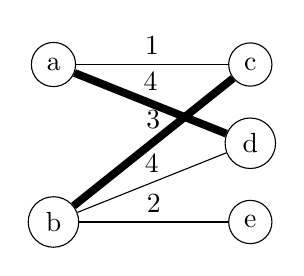
\begin{tikzpicture}
   \node[shape=circle,draw=black] (B) at (0,1) {b};
    \node[shape=circle,draw=black] (A) at (0,3) {a};
    \node[shape=circle,draw=black] (E) at (2.5,1) {e};
    \node[shape=circle,draw=black] (D) at (2.5,2) {d}; 
    \node[shape=circle,draw=black] (C) at (2.5,3) {c};

    \path[-] (A) edge node[above] {$1$} (C);
    \path [line width=1mm,-](A) edge node[above] {$4$} (D);
    \path [line width=1mm,-](B) edge node[above] {$3$} (C);
    \path [-](B) edge node[above] {$2$} (E);
    \path [-](B) edge node[above] {$4$} (D);

\end{tikzpicture}
\caption{This matching has a blocking pair $ac$.}
\end{figure}
\end{frame}

\begin{frame}
\frametitle{A Linear Programming Relaxation}
Let $LP_{SM}(G)$ be defined as follows:
\begin{align*}
&\text{maximize} &\sum_{e \in E} c_e x_e \\
&\text{subject to} &x(\delta(v)) &\leq 1, &\forall v \in V\\
& &\alert{x(\delta^{>w}(v))} \alert{+ x(\delta^{>v}(w)) + x_{vw}} &\alert{\geq 1,} &\alert{\forall vw \in E}\\
& &x_e &\geq 0, &\forall e \in E
\end{align*}
Let $n^*(x,v)$ ($n_*(x,v)$ respectively) be most (least respectively) preferred neighbour of $v$ such that $x_{vn^*(x,v)} > 0$ ($x_{vn_*(x,v)} > 0$ respectively). \\
Also define $S(x) = \{ v \in V : x(\delta(v)) > 0 \}$.
\end{frame}

\subsection{Some Observations}
\begin{frame}
\frametitle{Integral Points are Stable}
Let $x$ be the incidence vector of a matching on $G$. Then $x$ is stable if and only if $x$ is feasible for $LP_{SM}(G)$.\\
$\textbf{Proof Idea:}$ Since $x$ is integral, $x$ is infeasible if and only if there exists $vw \in E$ such that $$ x(\delta^{>w}(v)) = x(\delta^{>v}(w)) = x_{vw} = 0. $$
Such a $vw$ is a blocking pair. $\blacksquare$
\end{frame}

\begin{frame}
\frametitle{Lemma 1}
Let $x$ be feasible for $LP_{SM}(G)$ and let $vw \in E$. Then $$ v \not\in S(x) \text{ or } (v \in S(x) \text{ and } w \geq_v n^*(x,v)) $$ $\implies$ $$ x(\delta(w)) = 1 \text{ and } v \leq_w n_*(x,w). $$\\
$\textbf{Proof Idea:}$ In either case $x(\delta^{>w}(v)) = 0$. So $$1 \leq x(\delta^{>w}(x)) + x(\delta^{>v}(w)) + x_{vw} = x(\delta^{\geq v}(w)) \leq 1. \blacksquare$$\\
$\textbf{Note:}$ If $x(\delta^{>w}(v)) + x(\delta^{>v}(w)) + x_{vw} = 1$ then converse holds as well.
\end{frame}

\begin{frame}
\frametitle{Lemma 2}
Let $x$ be feasible for $LP_{SM}(G)$ and let $vw \in E$. Then $$v \in S(x) \text{ and } w = n^*(x,v)$$ if and only if $$x(\delta(w)) = 1 \text{ and } v = n_*(x,w). $$\\
$\textbf{Proof Idea:}$ Similar to previous with equality holding throughout. $\blacksquare$
\end{frame}

\begin{frame}
\frametitle{Lemma 3}
Let $x$ be feasible for $LP_{SM}(G)$. Then $$ v \in S(x) $$ if and only if $$x(\delta(v)) = 1.$$ \\
$\textbf{Proof Idea:}$
\begin{itemize}
\item By previous Lemmas $n(x,\cdot) : S(x) \rightarrow F(x) = \{v \in S(x) : x(\delta(v)) = 1 \}$.
\item If $n^*(x,v_1) = w = n^*(x,v_2)$ then by Lemma $2$ $v_1 = n_*(x,w) = v_2$
\item So $n^*(x,\cdot)$ is injective. $\blacksquare$
\end{itemize}
\end{frame}

\subsection{Rothblum's Original Proof}
\begin{frame}
\frametitle{Proof of Integrality}
Rothblum showed that the extreme points of  $LP_{SM}(G)$:
\begin{align*}
&\text{maximize} &\sum_{e \in E} c_e x_e \\
&\text{subject to} &x(\delta(v)) &\leq 1, &\forall v \in V\\
& &x(\delta^{>w}(v)) + x(\delta^{>v}(w)) + x_{vw} &\geq 1, &\forall vw \in E\\
& &x_e &\geq 0, &\forall e \in E
\end{align*}
are exactly its integral points.\\
$(\implies)$ If $x$ integral optimal solution to $LP_{SM}(G)$ then $x$ is extreme since the solutions of $LP_{SM}(G)$ are contained in the solutions of $LP_M(G)$.
\end{frame}

\begin{frame}
\frametitle{Proof of Integrality - Strategy}
$(\impliedby)$ Suppose $x$ is extreme point of $LP_{SM}(G)$. Rothblum uses a convex combination argument: 
\begin{itemize}
\item $x$ is extreme $\iff$ there does not exist $x^1 \neq x^2$ feasible such that $x = \frac{1}{2}(x^1 + x^2)$.
\item Define vector $z$ such that $z = 0$ $\implies$ $n^*(x,v) = n_*(x,v)$ for all $v$.
\item Which would imply $x$ is integral.
\item Rothblum then shows $x \pm \epsilon z$ feasible for sufficiently small $\epsilon$.
\item By extremality of $x$ proof is complete.
\end{itemize}
\end{frame}

\begin{frame}
\frametitle{Proof of Integrality - Definition of $z$}
Define the vectors $z^*$, $z_*$, and $z$ as follows:
\begin{align*}
(z^*)_{vw} &= \begin{cases}
	1, &\text{if $v\in S(x) \cap V_0$ and $w = n^*(x,v)$} \\
	0, &\text{otherwise}
\end{cases} 
\\
\uncover<2->{(z_*)_{vw} &= \begin{cases}
	1, &\text{if $v\in S(x) \cap V_0$ and $w = n_*(x,v)$} \\
	0, &\text{otherwise}
\end{cases}}
\\
\uncover<3->{z_{vw} &= (z^*)_{vw} - (z_*)_{vw}.}
\end{align*}
\uncover<4->{By invoking our Lemmas, $z^*$ and $z_*$ are equivalently:
\begin{align*}
(z^*)_{vw} &= \begin{cases}
	1, &\text{if $w\in S(x) \cap V_1$ and $v = n_*(x,w)$} \\
	0, &\text{otherwise}
\end{cases} 
\\
(z_*)_{vw} &= \begin{cases}
	1, &\text{if $w\in S(x) \cap V_1$ and $v = n^*(x,w)$} \\
	0, &\text{otherwise}
\end{cases}
\end{align*}}
\end{frame}

\begin{frame}
\frametitle{Proof of Integrality - Showing $x \pm \epsilon z$ is Feasible}
We claim that $z$ satisfies the following:
\begin{itemize}
\item<2-> If $x(\delta(v)) = 1$ then $z(\delta(v)) = 0$ for all $v \in V$.
\item<3-> If $x_e = 0$ then $z_e = 0$ for all $e \in E$.
\item<4-> If $x(\delta^{>w}(v)) + x(\delta^{>v}(w)) + x_{vw} = 1$ then $z(\delta^{>w}(v)) + z(\delta^{>v}(w)) + z_{vw} = 0$.
\end{itemize}
\uncover<5->{Thus we can choose $\epsilon > 0$ such that $x \pm \epsilon z$ is feasible for $LP_{SM}(G)$.} \\
\uncover<6->{Since $x$ is an extreme point this means $z = 0$. That is, $z^* = z_*$ and therefore $x$ is integral. $\blacksquare$}
\end{frame}

\section{An Iterative Rounding Proof?}
\subsection{Extreme Point Characterization}
\begin{frame}
Recall: $LP_{SM}(G)$:
\begin{align*}
&\text{maximize} &\sum_{e \in E} c_e x_e \\
&\text{subject to} &x(\delta(v)) &\leq 1, &\forall v \in V\\
& &x(\delta^{>w}(v)) + x(\delta^{>v}(w)) + x_{vw} &\geq 1, &\forall vw \in E\\
& &x_e &\geq 0, &\forall e \in E
\end{align*}
Is there an Iterative Rounding proof of integrality?\\
Recall Iterative Rounding: \\Characterize tight constraints $\Rightarrow$ Iterative Algorithm $\Rightarrow$ Analysis.
\end{frame}

\begin{frame}
\frametitle{Extreme Point Characterization}
Let $x$ be an extreme point solution to $LP_{SM}(G)$ such that $x>0$. Then there exists $W \subseteq V$ and \alert{$T \subseteq E$} such that the following hold:
\begin{enumerate}
\item $x(\delta(v)) = 1$, $\forall v \in W$.
\item\alert<1->{ $x(\delta^{>w}(v))+ x(\delta^{>v}(w) + x_{vw} = 1$, $\forall vw \in T$.}
\item The vectors in $\{\chi(\delta(v)) : v \in W\}$ together with the vectors in \alert<1->{$\{\chi(\delta_v^>(w)) + \chi(\delta_w^>(v)) + \chi(vw) : vw \in T\}$} are all linearly independent.
\item $|W| \alert{+ |T|} = |E|$.
\end{enumerate}
\end{frame}

\subsection{Finding a $0$ or $1$}

\begin{frame}
\frametitle{Finding a $0$ or $1$ - Choose $W$ and $T$}
\begin{itemize}
\item Suppose for a contradiction we have an extreme point solution of $LP_{SM}(G)$, $x$, such that $0 < x < 1$. 
\item There are $W \subseteq V$ and $T \subseteq E$ corresponding to a maximal set of linearly independent tight constraints such that $|W| + |T| = |E|$
\item Choose the pair $(W,T)$ which  maximizes $|W|$
\end{itemize}
\end{frame}

\begin{frame}
\frametitle{Finding a $0$ or $1$ - $vn_*(v) \not\in T$}
Let $v \in W$.  Let $w = n_*(v)$. Then $vw \not\in T$.\\
$\textbf{Proof Idea:}$
\begin{itemize}
\item<2-> If $vw$ in $T$ then $x(\delta^{>w}(v)) + x(\delta^{>v}(w)) + x_{vw} = 1 = x(\delta(v))$.
\item<3-> Since $\delta^{\geq w}(v) = \delta(v)$, we have $x(\delta^{>v}(w)) = 0$.
\item<4-> Therefore $\chi(\delta^{>w}(v)) + \chi(\delta^{>v}(w)) + \chi(vw) = \chi(\delta(v))$. This contradicts the linear independence of the constraints chosen.
\end{itemize}
\end{frame}

\begin{frame}
\frametitle{Finding a $0$ or $1$ - $vn^*(v) \not\in T$}
 Let $v \in V$. Let $w = n^*(v)$. Then $vw \not\in T$.\\
 $\textbf{Proof Idea:}$
\begin{itemize}
\item<2-> If $vw \in T$ then $x(\delta^{>w}(v)) + x(\delta^{>v}(w)) + x_{vw} = 1$.
\item<3-> Since $x(\delta^{>w}(v)) = 0$ we have $x(\delta^{\geq v}(w)) = 1$.
\item<4-> So $\chi(\delta^{\geq v}(w)) = \chi(\delta(w))$ and $\chi(\delta^{>w}(v)) + \chi(\delta^{>v}(w)) + \chi(vw) = \chi(\delta(w)).$
\item<5-> If $w \in W$ this contradicts linear independence. Otherwise this contradicts the maximality of $W$.
\end{itemize}
\end{frame}

\begin{frame}
\frametitle{Finding a $0$ or $1$ - Degree Lower Bound}
\begin{itemize}
\item As before, for any $v \in W$, $d(v) \geq 2$.
\item $\textbf{Proof Idea:}$ $x(\delta(v)) = 1$ and $x_e < 1$ for each $e \in \delta(v)$ so $d(v) \geq 2$. 
\item Since $vn^*(v)$ and $vn_*(v)$ are not in $T$ each vertex in $W$ has two incident edges not in $T$.
\end{itemize}
\end{frame}

\begin{frame}
\frametitle{Finding a $0$ or $1$ - Token argument}
Give each edge in $E$ a token. Redistribute tokens as follows for any $vw \in E$:
\begin{enumerate}
\item If $vw \in T$ have $vw$ give itself token.
\item Otherwise if $v \in W$ have $vw$ give $\frac{1}{2}$ token to $v$, and if $w \in W$ have $vw$ give $\frac{1}{2}$ token to $w$.
\end{enumerate}
\begin{itemize}
\item<2-> Clearly each edge does not give away more than it has, and each edge in $T$ receives a token.
\item<3-> Each vertex in $W$ receives a token since there are at least two adjacent edges not in $T$. 
\item<4-> As in the bipartite matching argument, we can find $v \not\in W$ and the edge $vn^*(v)$ does not give away all of its token. 
\end{itemize}
\uncover<4->{A contradiction.$\blacksquare$}
\end{frame}
\subsection{Algorithm?}
\begin{frame}
\frametitle{Iterative Algorithm}
\begin{enumerate}
\item Input bipartite stable matching instance $G$
\item Set matching $M$ to $\emptyset$
\item While $E \neq \emptyset$
\begin{enumerate}
\item Find extreme point optimal solution $x$ to $LP_M(G)$.
\item For each $e=vw \in E$ such that $x_e = 1$ add $e$ to $M$ and remove vertices $v,w$ from $G$.
\item For each $e \in E$ such that $x_e = 0$ remove $e$ from $G$.
\end{enumerate}
\item Output $M$
\end{enumerate}
\uncover<2->{But this doesn't work!\\ $LP_{SM}(G-e)$ loses stability constraint for $e$. So stable matching returned by algorithm on $G-e$, $M'$, comes with no guarantee that $M' \cup \{e\}$ is a stable matching on $G$}
\end{frame}
\begin{frame}
\frametitle{Can We Fix The Algorithm? - Edges of value $1$}
When we find $x_{vw} = 1$ we can be clever and do the following:
\begin{enumerate}
\item $\forall u \in N(v)$ (the neighbourhood of $v$) such that $v$ prefers $u$ to $w$ remove every edge in $\delta_u^<(v)$ from $G$
\item $\forall u \in N(w)$ such that $w$ prefers $u$ to $v$ remove every edge in $\delta_u^<(w)$ from $G$.
\item Remove $v, w$ from $G$.
\end{enumerate}
It can be shown that this ensures the matching returned on the residual graph plus edge $vw$ is a stable matching on $G$.\end{frame}
\begin{frame}
\frametitle{Can We Fix The Algorithm? - Edges of value $0$}
Unfortunately it is not clear what to do in the case where edges of value $0$ are found.\\
Questions to think about:
\begin{itemize}
\item Can we guarantee an edge of value $1$ to avoid this?
\item Is there a clever set of edges to remove alongside a $0$ edge to ensure the algorithm works?
\end{itemize}
\end{frame}
\section{References}
\begin{frame}
\frametitle{References}
\begin{enumerate}
\item Rothblum, Uriel G. "Characterization of stable matchings as extreme points of a polytope." $\textit{Mathematical Programming}$ 54.1-3 (1992): 57-67.
\item Lau, Lap Chi, Ramamoorthi Ravi, and Mohit Singh. $\textit{Iterative methods in combinatorial optimization}$. Vol. 46. Cambridge University Press, 2011
\end{enumerate}
\end{frame}
\end{document}
